\documentclass[10pt]{article}
\usepackage[a4paper,margin=20mm]{geometry}
\usepackage[T1]{fontenc}
\usepackage[utf8]{inputenc}
\usepackage{lmodern}
\usepackage{microtype}
\usepackage{amsmath,amssymb,bm}
\usepackage{booktabs,tabularx,array,multirow}
\usepackage{graphicx}
\usepackage{xcolor}
\usepackage{tikz}
\usetikzlibrary{arrows.meta,positioning,fit,calc,shapes.geometric,backgrounds}
\usepackage{pgfplots}
\pgfplotsset{compat=1.18}
\usepackage{enumitem}
\usepackage{caption}
\usepackage{subcaption}
\usepackage{siunitx}
\usepackage{natbib}
\usepackage{hyperref}
\usepackage{cleveref}
\usepackage{fancyhdr}
\usepackage{titlesec}
\usepackage{balance}

\definecolor{navy}{HTML}{17324D}
\definecolor{teal}{HTML}{138A8A}
\definecolor{amber}{HTML}{D99828}
\definecolor{redx}{HTML}{B24A4A}
\definecolor{greenx}{HTML}{3B8C61}
\definecolor{papergray}{HTML}{F2F4F5}
\definecolor{inkgray}{HTML}{4A5660}
\hypersetup{colorlinks=true,linkcolor=navy,citecolor=teal,urlcolor=teal,pdfauthor={Francisco Angulo de Lafuente},pdftitle={Audio-Frequency Microcoil Sensing for Flexible Robotic Skins}}
\pagestyle{fancy}
\fancyhf{}
\lhead{Sensory Skin Lab --- Preprint}
\rhead{Angulo de Lafuente}
\cfoot{\thepage}
\setlength{\headheight}{14pt}
\titleformat{\section}{\large\bfseries\color{navy}}{\thesection}{0.6em}{}
\titleformat{\subsection}{\normalsize\bfseries\color{teal}}{\thesubsection}{0.55em}{}
\setlist[itemize,enumerate]{nosep,leftmargin=*}
\newcommand{\R}{\mathbb{R}}
\newcommand{\dataset}{\textsc{SSkin-Pilot}}

\title{\vspace{-1.2cm}\textbf{Audio-Frequency Microcoil Sensing for Proximity, Material Response, and Contact Pressure in Flexible Robotic Skins}\\[0.45em]
\large A Research Platform, Exploratory Evidence Audit, and Prospective Validation Protocol}
\author{Francisco Angulo de Lafuente\\\small Independent Researcher, Spain}
\date{Revised preprint --- 25 August 2026}

\begin{document}
\maketitle
\begin{abstract}
Robotic skin requires compliant, distributed sensing that can support both gentle pre-contact interaction and contact-level material response. This paper presents \emph{Sensory Skin Lab}, an open browser-based research platform for evaluating fine copper microcoils intended for encapsulation in silicone-like flexible substrates. The system generates audio-band continuous or gated excitation, acquires a receive channel through a commodity audio interface, extracts amplitude, phase, transient, noise, and saturation features, and provides transparent empirical calibration for target response and \SIrange{0}{15}{\centi\metre} proximity. We position the concept relative to capacitive electronic skin, magnetic tactile skin, flexible inductive sensors, and magnetic-induction tomography. We then audit a set of uncontrolled pilot observations: strong response to a nearby human hand/body, weaker response to a ferrous pan, little apparent response to wood or plastic, persistence through an approximately \SI{5}{\centi\metre} wooden barrier, and dependence on software excitation settings even when the physical output path was disconnected. These observations demonstrate a detectable signal but do \emph{not} establish electromagnetic material discrimination or through-wall sensing, because body capacitance, codec DAC--ADC leakage, common power/ground modulation, automatic gain control, and motion remain viable explanations. Accordingly, no retrospective accuracy or range claim is made. We further formulate a continuous proximity--contact--force--pressure transducer in which elastomer compression changes microcoil geometry and coupling, and propose a lightweight uncertainty-aware multitask model that jointly estimates target class, distance, contact state, normal force, contact area, and pressure. The primary contribution is a falsifiable measurement model and a preregistered-style prospective protocol using isolated transmit and receive chains, instrumented indentation, non-conductive positioning, randomized blocked trials, negative controls, held-out objects and skin batches, and explicit success thresholds. The resulting platform is suitable for disciplined feasibility studies on low-cost microcoil arrays while preserving a clear boundary between demonstration, hypothesis, and validated robotic-safety performance.
\end{abstract}

\noindent\textbf{Keywords:} electronic skin; robotic skin; microcoil; inductive sensing; proximity sensing; magnetic induction; human--robot interaction; Web Audio; reproducible experimentation.

\vspace{0.6em}
\noindent\colorbox{papergray}{\parbox{0.97\linewidth}{\textbf{Evidence status.} This manuscript reports a software/hardware research design and qualitative exploratory observations. It contains no controlled performance dataset and makes no validated claim of material classification, absolute range, through-wall imaging, or safety certification. All numerical success criteria in \cref{sec:protocol} are prospective.}}

\section{Introduction}
Human skin integrates dense mechanoreception with compliance, distributed geometry, and continuous feedback. Robotic equivalents remain difficult because area, wiring, stretch, hysteresis, calibration, energy, and robustness must be solved simultaneously \citep{dahiya2010tactile,hammock2013evolution,chortos2016prosthetic}. Large-area capacitive systems have demonstrated scalable tactile coverage \citep{someya2004large,maiolino2013capacitive}, while multimodal modules and neuromorphic afferent pathways show how local transducers can become useful perception systems \citep{mittendorfer2011humanoid,tee2015mechanoreceptor,kim2018afferent}. Yet physical human--robot interaction benefits from sensing before contact as well as during contact: a robot that estimates approach over the final centimetres can reduce speed before a handover, handshake, or incidental collision \citep{pang2018flexible,fonseca2023hybrid}.

This work investigates whether fine, inexpensive copper coils embedded in a compliant skin can form an additional sensing modality. The motivating vision is not a single ``metal detector'' attached to a robot, but a distributed array whose frequency-dependent electromagnetic response may complement force, vision, and joint-torque sensing. Inductive approaches are attractive because the conductors can be sealed, interrogation can be contactless, and coil geometry is compatible with flexible circuits or enamelled wire. Their interpretation is nevertheless difficult. The measured voltage may combine true target interaction with direct transmitter--receiver coupling, electric-field coupling to a human body, mechanical deformation of the coil, acoustic microphonics, and electronic leakage inside the audio interface.

We make five contributions:
\begin{enumerate}
  \item an open, resource-conscious browser instrument for controlled audio-frequency excitation, feature extraction, calibration, and CSV logging;
  \item a physics-based measurement model that exposes alternative signal paths rather than treating any response as target detection;
  \item an explicit evidence audit of the existing pilot observations, separating observation from interpretation; and
  \item a prospective, preregistered-style protocol for evaluating proximity estimation and three-way target-response discrimination without operator-body leakage.
  \item a physics-constrained multitask-AI design and calibration protocol for the final centimetre of approach, contact detection, normal-force estimation, contact-area inference, and pressure mapping.
\end{enumerate}

\section{Related Work and Research Gap}
\subsection{Flexible tactile and proximity skins}
Pressure-sensitive e-skins span piezoresistive, capacitive, piezoelectric, triboelectric, optical, and magnetic transduction \citep{hammock2013evolution,nguyen2022recent,roberts2021soft}. Microstructured dielectric layers can greatly improve capacitive pressure sensitivity \citep{mannsfeld2010pressure}, and hierarchical structures can resolve pressure direction \citep{boutry2018direction}. Systems such as ReSkin and AnySkin emphasize replaceability, transfer, and practical robot learning around magnetic skins \citep{bhirangi2022reskin,bhirangi2024anyskin}. These achievements concern contact-rich tactile sensing; pre-contact distance and material response remain a complementary problem.

Self-capacitive proximity sensing is mature and naturally sensitive to the human body. Fonseca \emph{et al.} combined self-capacitance with piezoresistance in a flexible interface and explicitly documented susceptibility to moving robot actuators \citep{fonseca2023hybrid}. The broader proximity-skin literature likewise stresses field geometry, parasitic capacitance, grounding, and environmental drift \citep{wu2024proximity}. This is directly relevant: a strong hand response is not diagnostic of inductive coupling because a hand is also a large lossy conductor capacitively coupled to ground.

\subsection{Magnetic and inductive skins}
Magnetic skins can infer contact force from deformation of magnets or magnetized films. Yan \emph{et al.} demonstrated force decoupling and learned super-resolution using a sinusoidally magnetized film and Hall sensing \citep{yan2021magnetic}; ReSkin uses a replaceable elastomeric magnetic medium over magnetometers \citep{bhirangi2022reskin}. These are deliberately magnetized tactile transducers, distinct from the passive target perturbation explored here.

Flexible coils offer another route. Peng \emph{et al.} combined a planar coil, porous ferrite, and soft conductive film, using two interrogation frequencies to decouple bending and force \citep{peng2024inductive}. Dingley \emph{et al.} used mutual-inductance arrays and tomography to reconstruct contact-related changes in an engineered skin medium \citep{dingley2023emskin}. Fabrication materials and geometry materially affect resonant-sensor quality \citep{wang2020resonant}. These studies establish that flexible inductive sensing is scientifically credible, but they do not validate arbitrary classification of remote human, metallic, and insulating targets using a commodity audio codec.

Learning-based tactile skins show that a compliant medium can encode force and contact location in a distributed field response. Hellebrekers \emph{et al.} used a soft magnetic composite and neural network for continuous force and location estimation \citep{hellebrekers2020force}; this is evidence for the general calibration strategy, not evidence that the present microcoil achieves the same performance. Multitask learning can share representations between related classification and regression targets \citep{caruana1997multitask}, while task-dependent uncertainty provides a principled way to balance losses with different units \citep{kendall2018uncertainty}. These methods motivate a single model spanning approach and contact, provided that force and pressure labels come from independent reference instruments.

\begin{table*}[t]
\centering\small
\caption{Representative state of the art and the gap addressed by this work. Reported capabilities belong to the cited systems; they are not performance claims for Sensory Skin Lab.}
\label{tab:sota}
\begin{tabularx}{\textwidth}{@{}p{2.2cm}p{2.2cm}X X p{2.4cm}@{}}
\toprule
Approach & Transduction & Strength & Principal confound/limitation & Relation to this work\\
\midrule
Large-area capacitive skin \citep{maiolino2013capacitive} & Capacitance & Scalable, compliant tactile coverage & Parasitics, grounding, wiring & Baseline architecture for distributed skin\\
Hybrid proximity/force \citep{fonseca2023hybrid} & Self-capacitance + piezoresistance & Pre-contact and contact in one layer & EMI and actuator-dependent errors & Closest functional target; motivates controls\\
ReSkin / AnySkin \citep{bhirangi2022reskin,bhirangi2024anyskin} & Magnetic elastomer + magnetometer & Replaceable, learnable tactile interface & Primarily contact; learned domain shift & Reference for dataset and transfer design\\
Soft magnetic skin \citep{yan2021magnetic} & Magnetized film + Hall array & Multi-axis force and learned resolution & Requires engineered magnetic layer & Demonstrates field-based tactile inference\\
Soft inductive bimodal sensor \citep{peng2024inductive} & Coil + ferrite + conductor & Two-wire bending/force decoupling & Engineered target layers; contact regime & Direct evidence for flexible-coil sensing\\
EM-skin tomography \citep{dingley2023emskin} & Mutual-inductance coil array & Spatial reconstruction and multi-touch & Dedicated multichannel hardware & Array-scale route beyond one coil\\
\textbf{Sensory Skin Lab} & Audio-band microcoil response & Open browser acquisition; explicit confound audit & Unvalidated pilot; commodity-codec leakage & Low-cost feasibility and controlled protocol\\
\bottomrule
\end{tabularx}
\end{table*}

The research question is therefore:
\begin{quote}
\emph{Can audio-frequency microcoil elements embedded in compliant substrates provide repeatable, separable feature signatures for human/biological, metallic, and non-conductive targets, support calibrated \SIrange{0}{15}{\centi\metre} proximity, and use contact-induced deformation to estimate normal force and average pressure under controlled suppression of capacitive, acoustic, mechanical-history, and electronic-crosstalk confounds?}
\end{quote}

\section{Physical Basis and Measurement Model}
\subsection{Inductive response}
For sinusoidal excitation at angular frequency $\omega$, a receive coil coupled to a transmit coil has the idealized open-circuit component
\begin{equation}
V_{\mathrm{rx}}(\omega)=j\omega M(\omega,\mathcal{T},\mathbf{r})I_{\mathrm{tx}}(\omega),
\label{eq:mutual}
\end{equation}
where $M$ is mutual inductance and depends on target properties $\mathcal{T}$ and position $\mathbf{r}$. A conductive target supports eddy currents that oppose the incident field and perturb both loss and apparent inductance. A magnetic target may also alter flux through permeability. In a real system the coil impedance is $Z_c=R_c+j\omega L_c$ with parasitic capacitance and frequency-dependent losses.

For a homogeneous conductor, the plane-wave skin depth is
\begin{equation}
\delta=\sqrt{\frac{2}{\omega\mu\sigma}},
\label{eq:skin}
\end{equation}
where $\mu$ and $\sigma$ are permeability and conductivity. Although near-field coil geometry is not a plane wave, \cref{eq:skin} gives an important qualitative constraint: higher frequency normally \emph{reduces} penetration into a good conductor. Frequency can still improve measured sensitivity by increasing induced voltage, eddy-current strength, or receiver signal-to-noise ratio. Those mechanisms must not be conflated with penetration.

\begin{figure}[t]
\centering
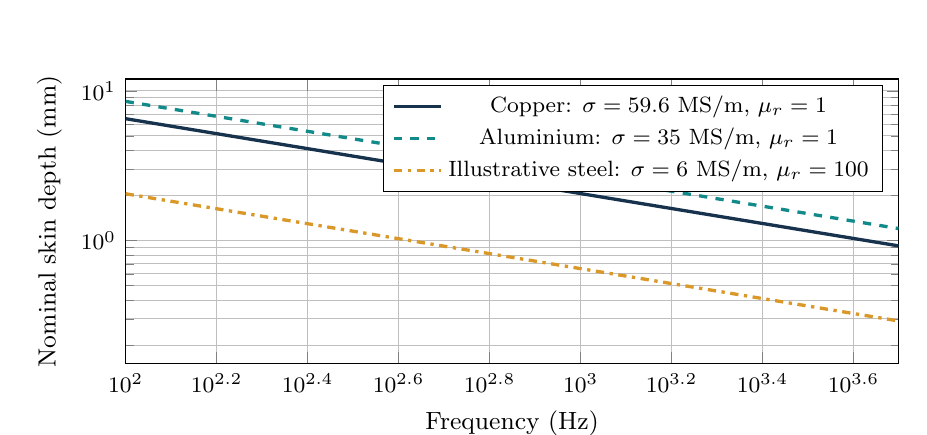
\begin{tikzpicture}
\begin{axis}[
 width=.94\linewidth,height=5.2cm,
 xmode=log,ymode=log,xmin=100,xmax=5000,ymin=.15,ymax=12,
 xlabel={Frequency (Hz)},ylabel={Nominal skin depth (mm)},
 grid=both,legend style={font=\footnotesize,at={(0.98,0.98)},anchor=north east},
 tick label style={font=\footnotesize},label style={font=\small}]
\addplot[navy,very thick,domain=100:5000,samples=80] {1000*sqrt(2/(2*pi*x*4*pi*1e-7*5.96e7))};
\addlegendentry{Copper: $\sigma=59.6$ MS/m, $\mu_r=1$}
\addplot[teal,very thick,dashed,domain=100:5000,samples=80] {1000*sqrt(2/(2*pi*x*4*pi*1e-7*3.5e7))};
\addlegendentry{Aluminium: $\sigma=35$ MS/m, $\mu_r=1$}
\addplot[amber,very thick,dashdotted,domain=100:5000,samples=80] {1000*sqrt(2/(2*pi*x*4*pi*1e-7*100*6e6))};
\addlegendentry{Illustrative steel: $\sigma=6$ MS/m, $\mu_r=100$}
\end{axis}
\end{tikzpicture}
\caption{Analytical skin-depth curves from \cref{eq:skin}; these are calculations, not measurements. Steel permeability is strongly alloy-, field-, and frequency-dependent, so the steel curve is illustrative only.}
\label{fig:skin}
\end{figure}

\subsection{Competing signal paths}
The digitized sample is better represented as a superposition:
\begin{align}
y(t)={}&h_{\mathrm{em}}(\mathcal{T},\mathbf{r})*s(t)+h_{\mathrm{direct}}*s(t)+h_{\mathrm{codec}}*s(t) \nonumber\\
&+h_{\mathrm{cap}}(\mathbf{b},g)*s(t)+h_{\mathrm{mech}}*a(t)+n(t),
\label{eq:model}
\end{align}
where $h_{\mathrm{em}}$ is target-dependent electromagnetic coupling, $h_{\mathrm{direct}}$ is direct coil/cable coupling, $h_{\mathrm{codec}}$ is electronic DAC--ADC or power/ground leakage, $h_{\mathrm{cap}}$ represents body/environment capacitance as a function of body configuration $\mathbf{b}$ and grounding $g$, $a(t)$ is vibration/acoustic excitation, and $n(t)$ is noise and drift. A useful experiment must identify $h_{\mathrm{em}}$ while controlling or estimating the other terms.

\begin{figure*}[t]
\centering
\resizebox{\textwidth}{!}{%
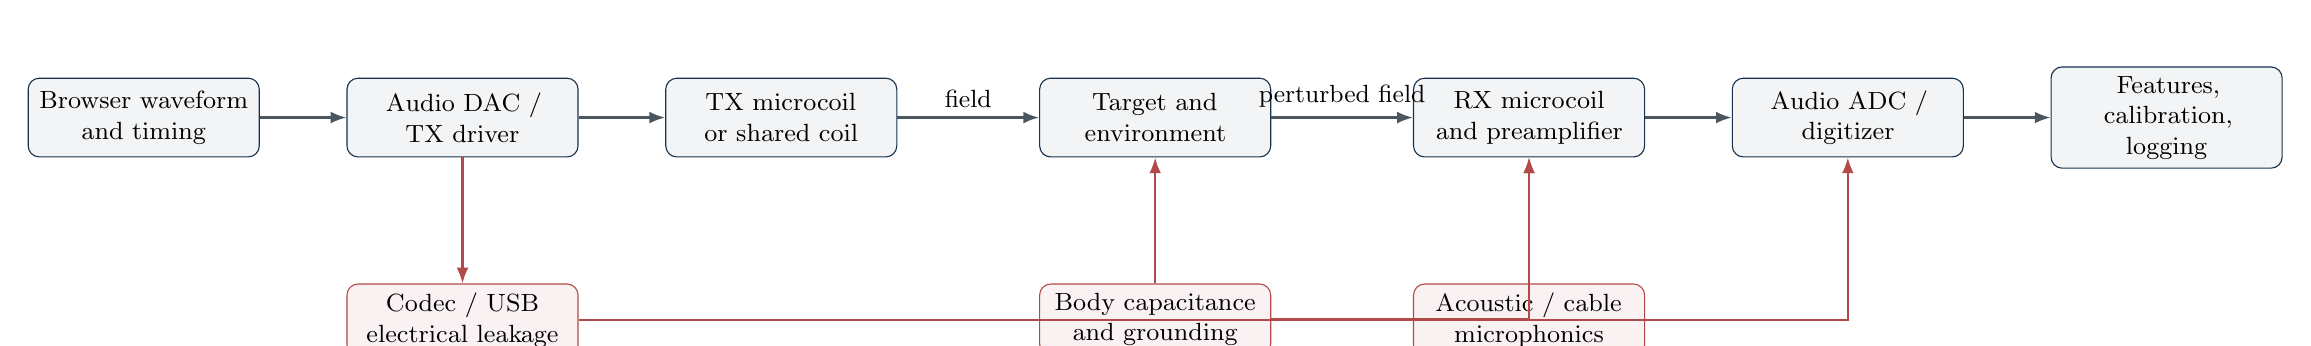
\begin{tikzpicture}[font=\small, node distance=8mm and 11mm,
 box/.style={draw=navy,rounded corners,fill=papergray,minimum height=10mm,align=center,text width=27mm},
 risk/.style={draw=redx,rounded corners,fill=redx!7,minimum height=9mm,align=center,text width=27mm},
 arr/.style={-{Latex[length=2mm]},thick,draw=inkgray}]
\node[box] (web) {Browser waveform\\and timing};
\node[box,right=of web] (dac) {Audio DAC /\\TX driver};
\node[box,right=of dac] (tx) {TX microcoil\\or shared coil};
\node[box,right=18mm of tx] (target) {Target and\\environment};
\node[box,right=18mm of target] (rx) {RX microcoil\\and preamplifier};
\node[box,right=of rx] (adc) {Audio ADC /\\digitizer};
\node[box,right=of adc] (dsp) {Features, calibration,\\logging};
\draw[arr] (web)--(dac); \draw[arr] (dac)--(tx); \draw[arr] (tx)--node[above]{field}(target); \draw[arr] (target)--node[above]{perturbed field}(rx); \draw[arr] (rx)--(adc); \draw[arr] (adc)--(dsp);
\node[risk,below=16mm of dac] (leak) {Codec / USB\\electrical leakage};
\node[risk,below=16mm of target] (body) {Body capacitance\\and grounding};
\node[risk,below=16mm of rx] (micro) {Acoustic / cable\\microphonics};
\draw[arr,redx] (dac)--(leak); \draw[arr,redx] (leak.east)-| (adc.south);
\draw[arr,redx] (body)--(target); \draw[arr,redx] (body.east)-| (rx.south);
\draw[arr,redx] (micro)--(rx);
\end{tikzpicture}
}
\caption{System architecture and causal confounds. Red paths can produce apparent ``detection'' without a target-specific inductive mechanism. The validation protocol isolates or randomizes these paths.}
\label{fig:architecture}
\end{figure*}

\subsection{Contact mechanics and pressure observability}
Once the remaining gap closes and the target indents the encapsulant, the sensor enters a second physical regime. Let $h_0$ be unloaded skin thickness and $u(t)$ indentation. Engineering compressive strain is $\varepsilon(t)=u(t)/h_0$. The local normal force and area-averaged pressure satisfy
\begin{equation}
F_n(t)=\int_{A_c(t)}p(\mathbf{r},t)\,\mathrm{d}A,\qquad \bar p(t)=\frac{F_n(t)}{A_c(t)},
\label{eq:pressure}
\end{equation}
where $A_c$ is the instantaneous contact area. A single scalar coil response cannot uniquely determine both $F_n$ and $A_c$ without extra geometry, an array, or a learned prior. Consequently, a single cell can report force or \emph{average} pressure only for calibrated indenters or a constrained effective area; spatial pressure requires multiple cells and contact-area reconstruction.

Compression can change the coil's area, turn spacing, distance to a target, parasitic capacitance, resistance, and mutual inductance. A useful local model is
\begin{equation}
\Delta\mathbf{z}(t)=\mathcal{H}\!\left(\mathcal{T},d(t),\varepsilon(t),\dot\varepsilon(t),T(t),\mathbf{s}(t);\boldsymbol\theta_{\mathrm{skin}}\right)+\boldsymbol\eta(t),
\label{eq:contactmodel}
\end{equation}
where $\mathbf{s}$ is deformation history and $\boldsymbol\theta_{\mathrm{skin}}$ includes thickness, hardness, batch, cure, coil geometry, and compression response. Density and a nominal elastic modulus are insufficient: silicone and latex-like elastomers exhibit nonlinear stress--strain response, hysteresis, creep, stress relaxation, temperature dependence, and permanent-set or ageing effects. Compression specimens should be characterized independently using a defined procedure such as ISO~7743 \citep{iso7743}; the assembled skin then requires its own cyclic calibration.

The proposed operating continuum has three regimes: (i) \emph{pre-contact}, in which distance and target-response features dominate; (ii) \emph{transition}, approximately the final centimetre in the present hypothesis, in which field response and initial deformation coexist; and (iii) \emph{contact}, in which deformation-sensitive features support force inference. The regime boundaries are sensor- and target-specific and must be learned from synchronized displacement and load references rather than fixed retrospectively.

\section{Sensory Skin Lab Platform}
\subsection{Design goals and implementation}
Sensory Skin Lab is a client-side application implemented with TypeScript, React, and the Web Audio API \citep{sensoryskin2026software}. Audio samples are processed locally in an \texttt{AudioWorklet}; the application does not upload audio. The architecture was chosen for reproducibility and accessibility on commodity laptops and mobile browsers, not for metrology-grade timing. The interface supports:
\begin{itemize}
  \item passive receive, continuous VLF, and gated burst/PI-like excitation;
  \item identical mono excitation on the left and right output channels;
  \item user controls for frequency, output level, sensitivity, threshold, burst duration, listen delay, and phase weight;
  \item empty-field baseline acquisition and automatic saturation indication;
  \item real-time amplitude, phase, transient-decay, noise, clipping, and combined-response metrics;
  \item empirical reference capture for human/biological, metallic, and non-conductive classes;
  \item proximity anchors at \SIlist{15;10;5;2;0}{\centi\metre}; and
  \item five-sample-per-second CSV logging for offline analysis.
\end{itemize}

Browser audio stacks may apply undocumented resampling, gain, echo cancellation, noise suppression, or device routing. Constraints should be requested where supported, but every recorded session must log the browser, operating system, interface, nominal and realized sample rates, device identifiers, and whether signal enhancement is disabled.

\subsection{Feature representation}
For a measurement window $x[n]$ and baseline $x_0[n]$, the platform computes interpretable components rather than a black-box score. At the commanded frequency $f_0$, complex demodulation gives
\begin{equation}
X(f_0)=\frac{2}{N}\sum_{n=0}^{N-1}x[n]w[n]e^{-j2\pi f_0n/f_s}.
\end{equation}
The amplitude residual and wrapped phase displacement are
\begin{equation}
\Delta A_{\mathrm{dB}}=20\log_{10}\frac{|X|+\epsilon}{|X_0|+\epsilon},\qquad
\Delta\phi=\mathrm{wrap}(\angle X-\angle X_0).
\end{equation}
For gated excitation, a transient descriptor compares energy in a configured post-blanking window with baseline energy. Noise is estimated outside the driven band, and clipping is determined from sample occupancy near full scale. The feature vector is
\begin{equation}
\mathbf{z}=[|\Delta A_{\mathrm{dB}}|,\ |\Delta\phi|,\ |\Delta E_{\mathrm{tr}}|,\ \Delta N,\ q_{\mathrm{clip}}]^{\top}.
\end{equation}
Saturated or invalid components are excluded from the combined score rather than allowed to dominate it. Adaptive ground/baseline tracking may update only in stable, target-free intervals and must freeze on threshold crossings.

The demonstration classifier stores a centroid $\bm\mu_k$ for each user-captured class and assigns the nearest standardized centroid. Its displayed confidence is a relative separation between the smallest and second-smallest distances; it is not a calibrated posterior probability. For proximity, response strength is interpolated between target-specific anchors. Non-monotonic anchors must invalidate the distance display.

\subsection{Proposed microcoil skin construction}
The first physical demonstrator should use enamelled copper wire or a flexible printed spiral on a mechanically defined carrier, followed by separately cast silicone encapsulation. Direct co-printing of bare copper and ``silicone-like'' filament is not assumed to preserve insulation, trace position, or biocompatibility. The coil record must include wire diameter, turns, inner/outer diameter, DC resistance, inductance, quality factor, self-resonant frequency, encapsulant, thickness, bend radius, strain history, and temperature rise.

\begin{figure}[t]
\centering
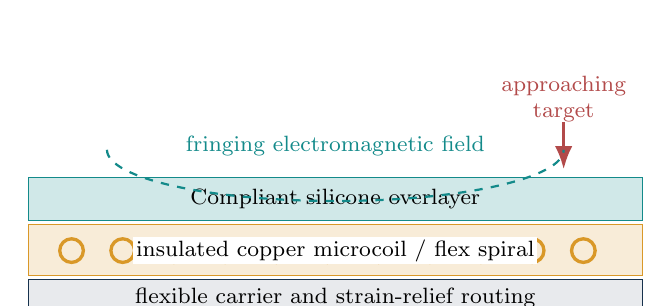
\begin{tikzpicture}[x=1cm,y=1cm,font=\footnotesize]
\fill[teal!20] (0,0) rectangle (7.8,.55); \draw[teal] (0,0) rectangle (7.8,.55);
\node at (3.9,.275) {Compliant silicone overlayer};
\fill[amber!18] (0,-.7) rectangle (7.8,-.05); \draw[amber] (0,-.7) rectangle (7.8,-.05);
\foreach \x in {.55,1.2,...,7.35}{\draw[amber,very thick] (\x,-.38) circle (.15);}
\node[fill=white,inner sep=1pt] at (3.9,-.38) {insulated copper microcoil / flex spiral};
\fill[navy!10] (0,-1.2) rectangle (7.8,-.75); \draw[navy] (0,-1.2) rectangle (7.8,-.75);
\node at (3.9,-.98) {flexible carrier and strain-relief routing};
\draw[redx,very thick,-{Latex}] (6.8,1.25)--(6.8,.65); \node[redx,align=center] at (6.8,1.55) {approaching\\target};
\draw[teal,dashed,thick] (1,.9) arc[start angle=180,end angle=360,x radius=2.9,y radius=.65];
\node[teal] at (3.9,.95) {fringing electromagnetic field};
\end{tikzpicture}
\caption{Proposed sensor stack. Independent force/contact sensing, electrical isolation, and temperature monitoring remain required for human-facing robotics.}
\label{fig:stack}
\end{figure}

\section{Proposed Multitask Perception System}
\label{sec:ai}
\subsection{Outputs and operational definitions}
The intended skin is not a binary detector. Each cell or local array should produce a synchronized perceptual state
\begin{equation}
\hat{\mathbf{y}}_t=\{\hat c_t,\hat d_t,\hat q_t,\hat F_{n,t},\hat A_{c,t},\hat p_t,\hat{\mathbf{u}}_t\},
\end{equation}
where $c$ is target-response class, $d$ distance, $q$ contact probability, $F_n$ normal force, $A_c$ contact area, $p$ average pressure, and $\mathbf{u}$ contains predictive uncertainty and an out-of-distribution (OOD) score. ``Human'' is an operational response class learned from consented examples and validated phantoms, not a claim of biological identity. ``Non-conductive'' means no separable conductive/magnetic response within the validated operating domain, not proof of composition.

\begin{table*}[t]
\centering\small
\caption{Proposed outputs, independent labels, metrics, and validity gates. All targets are prospective.}
\label{tab:aioutputs}
\begin{tabularx}{\textwidth}{@{}p{2.2cm}p{3.1cm}X p{3.0cm}@{}}
\toprule
Output & Reference label & Reported metric & Gate for use\\
\midrule
Target response & Material record; saline phantom or consented adult hand & Object-grouped macro-$F_1$, sensitivity, specificity, calibration & Reject if OOD or dummy-load leakage is class-informative\\
Distance, 0--15 cm & Traceable translation stage & Median/95th-percentile absolute error; monotonicity violations & Pre-contact only; target-specific calibration valid\\
Contact state & Load cell threshold plus displacement/optical event & Balanced accuracy, false-contact and missed-contact rates, detection latency & Two independent references agree\\
Normal force & Calibrated load cell & MAE, normalized RMSE, 95th-percentile absolute error, hysteresis & Contact only; skin batch and temperature in domain\\
Contact area & Machine-vision footprint or known flat indenter & Area IoU or relative area error & Spatial array or constrained indenter geometry\\
Average pressure & $F_n/A_c$ from independent references & MAE and normalized RMSE by indenter and material & Both force and area gates pass\\
Uncertainty / OOD & Held-out people, objects, skin batches, temperatures, faults & Coverage, selective risk, false-reject rate & Unsafe/unknown maps to conservative robot action\\
\bottomrule
\end{tabularx}
\end{table*}

\subsection{Input representation and model architecture}
The input is a short causal sequence of raw or demodulated RX data synchronized with commanded TX current, plus temperature and cell identity. The feature tensor contains multi-frequency in-phase and quadrature components, amplitude residual, phase displacement, transient energies, harmonics, broadband noise, clipping, adjacent-cell coupling, and temporal derivatives. A measured TX-current reference is essential; commanded software amplitude is not a substitute.

A low-resource implementation uses a compact one-dimensional temporal convolutional network (TCN) or gated recurrent encoder shared by six heads. The class and contact heads use calibrated classification losses; distance, force, and area heads use robust regression losses; pressure is computed through the physics layer $\hat p=\hat F_n/(\hat A_c+\epsilon)$ rather than independently whenever area is observable. Task-uncertainty weighting follows the multitask principle of \citet{kendall2018uncertainty}:
\begin{equation}
\mathcal{L}=\sum_{k\in\mathcal{R}}\left(\frac{\mathcal{L}_k}{2\sigma_k^2}+\log\sigma_k\right)+\sum_{k\in\mathcal{C}}\left(\frac{\mathcal{L}_k}{\sigma_k^2}+\log\sigma_k\right)+\lambda_{\mathrm{phys}}\mathcal{L}_{\mathrm{phys}},
\label{eq:multiloss}
\end{equation}
where $\mathcal{R}$ and $\mathcal{C}$ denote regression and classification tasks. The physics-consistency term penalizes negative force/area, pressure--force inconsistency, a nonzero pressure prediction before contact, discontinuity at the regime transition, and implausible high-frequency force changes relative to the calibrated mechanical bandwidth.

\begin{figure*}[t]
\centering
\resizebox{\textwidth}{!}{%
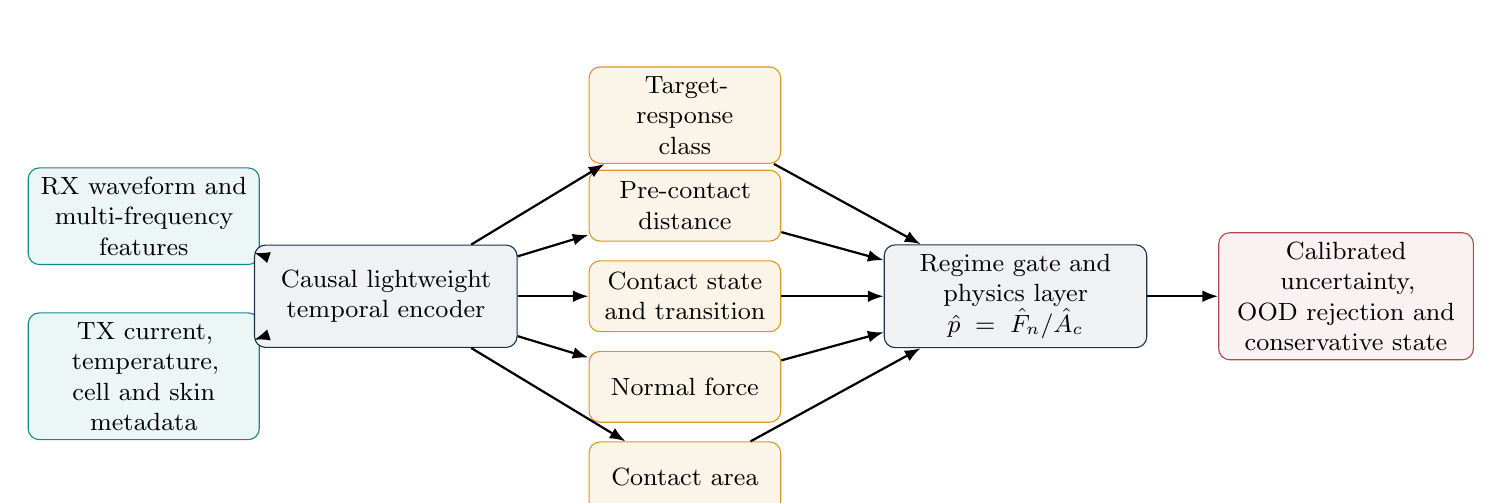
\begin{tikzpicture}[font=\small,node distance=6mm and 9mm,
 io/.style={draw=teal,rounded corners,fill=teal!8,align=center,text width=27mm,minimum height=11mm},
 core/.style={draw=navy,rounded corners,fill=navy!7,align=center,text width=31mm,minimum height=13mm},
 head/.style={draw=amber,rounded corners,fill=amber!10,align=center,text width=22mm,minimum height=9mm},
 safe/.style={draw=redx,rounded corners,fill=redx!7,align=center,text width=30mm,minimum height=11mm},
 arr/.style={-{Latex[length=2mm]},thick}]
\node[io] (rx) {RX waveform and\\multi-frequency features};
\node[io,below=of rx] (ref) {TX current, temperature,\\cell and skin metadata};
\node[core,right=14mm of $(rx)!0.5!(ref)$] (enc) {Causal lightweight\\temporal encoder};
\node[head,right=of enc,yshift=23mm] (class) {Target-response\\class};
\node[head,right=of enc,yshift=11.5mm] (dist) {Pre-contact\\distance};
\node[head,right=of enc] (contact) {Contact state\\and transition};
\node[head,right=of enc,yshift=-11.5mm] (force) {Normal force};
\node[head,right=of enc,yshift=-23mm] (area) {Contact area};
\node[core,right=13mm of contact] (physics) {Regime gate and\\physics layer\\$\hat p=\hat F_n/\hat A_c$};
\node[safe,right=of physics] (unc) {Calibrated uncertainty,\\OOD rejection and\\conservative state};
\draw[arr] (rx)--(enc); \draw[arr] (ref)--(enc);
\foreach \n in {class,dist,contact,force,area}{\draw[arr] (enc)--(\n); \draw[arr] (\n)--(physics);}
\draw[arr] (physics)--(unc);
\end{tikzpicture}}
\caption{Proposed shared-encoder multitask system. The pressure output is gated by independently validated contact, force, and area estimates. Unknown conditions do not receive an optimistic class or force value.}
\label{fig:ai}
\end{figure*}

\subsection{Uncertainty, rejection, and safe deployment}
Model confidence must not be interpreted as safety. Use deep ensembles or another validated epistemic-uncertainty method, calibrate classification probabilities on a validation set, and construct prediction intervals for distance and force. Conformal calibration may provide empirical coverage under exchangeability, but distribution shift can invalidate that premise. Recent uncertainty-aware robotic safety filters illustrate why OOD states must be detected rather than forced into a known label \citep{seo2025unisafe}. At runtime, high uncertainty, clipping, missing cells, temperature excursions, non-monotonic distance, or unrecognized skin metadata produce an \emph{unknown/degraded} state that commands reduced speed or a stop through an independent safety controller.

The software should deploy two layers: a transparent nearest-centroid or regularized linear baseline for diagnostics, and the frozen compact multitask model for validated operation. Quantization and bounded causal windows support phone-class or embedded hardware. The model artifact must be versioned with training-data hashes, sensor geometry, skin formulation, preprocessing, calibration temperatures, and approved operating domain.

\section{Exploratory Pilot Evidence Audit}
\label{sec:pilot}
\subsection{Provenance}
The pilot observations were generated during iterative, operator-led experimentation with a legacy detector coil plate, a small USB audio interface, and later a headphone-sized loudspeaker coil. Settings were changed adaptively, objects were often hand-held, the operator was not blinded, geometry was not fixed, and raw synchronized traces were not preserved as a controlled dataset. These conditions are useful for hypothesis generation but preclude inferential statistics, classifier accuracy, calibrated range, or causal attribution.

\subsection{Observed phenomena}
The stable claims are limited to what was directly noticed:
\begin{enumerate}
  \item the receive signal changed strongly when a hand or body approached, with apparent response extending from tens of centimetres to approximately one metre under selected settings;
  \item a ferrous pan produced a weaker but visible response;
  \item wood and plastic did not produce an obvious response once hand proximity was separated from the object presentation;
  \item hand and pan responses appeared similar when placed behind an approximately \SI{5}{\centi\metre} wooden board;
  \item lower audio frequencies, approximately \SIrange{120}{1000}{\hertz}, were qualitatively more useful; gated burst/PI-like operation appeared strongest, hybrid operation second, and continuous VLF weakest in the latest configuration; and
  \item frequency, output level, sensitivity, and threshold settings affected the received display even when the physical audio output was disconnected or routed to the laptop loudspeakers.
\end{enumerate}

\begin{figure}[t]
\centering
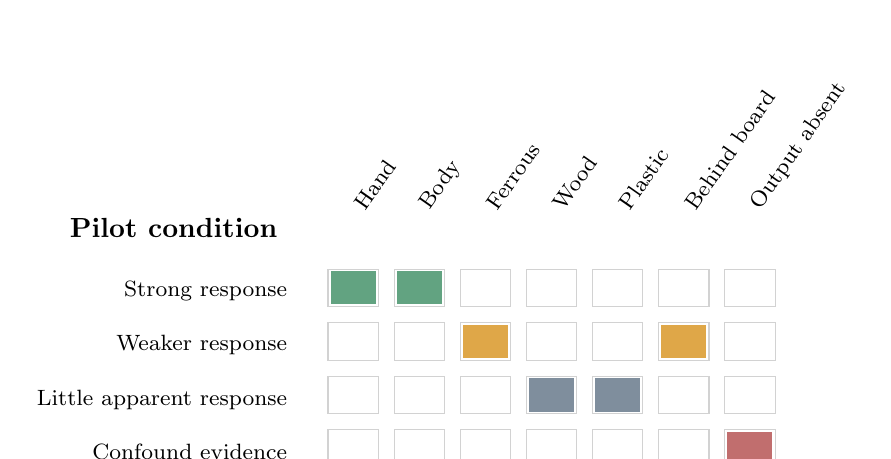
\begin{tikzpicture}[font=\footnotesize,x=.84cm,y=.68cm]
\node[anchor=e,font=\bfseries] at (0,4.2) {Pilot condition};
\foreach \x/\lab in {1/Hand,2/Body,3/Ferrous,4/Wood,5/Plastic,6/Behind board,7/Output absent}{\node[rotate=55,anchor=west] at (\x,4.35) {\lab};}
\foreach \y/\lab in {3/Strong response,2/Weaker response,1/Little apparent response,0/Confound evidence}{\node[anchor=e] at (.15,\y) {\lab};}
\foreach \x in {1,...,7}{\foreach \y in {0,...,3}{\draw[gray!35] (\x-.38,\y-.35) rectangle (\x+.38,\y+.35);}}
\fill[greenx!80] (1-.34,3-.31) rectangle (1+.34,3+.31);
\fill[greenx!80] (2-.34,3-.31) rectangle (2+.34,3+.31);
\fill[amber!85] (3-.34,2-.31) rectangle (3+.34,2+.31);
\fill[navy!55] (4-.34,1-.31) rectangle (4+.34,1+.31);
\fill[navy!55] (5-.34,1-.31) rectangle (5+.34,1+.31);
\fill[amber!85] (6-.34,2-.31) rectangle (6+.34,2+.31);
\fill[redx!80] (7-.34,0-.31) rectangle (7+.34,0+.31);
\end{tikzpicture}
\caption{Qualitative audit matrix. A colored cell records an operator observation, not a measured effect size. ``Behind board'' combines hand and ferrous-pan observations; ``output absent'' is evidence for an electronic or capacitive confound.}
\label{fig:audit}
\end{figure}

\subsection{Interpretation and competing hypotheses}
The observations are compatible with at least five hypotheses, which are not mutually exclusive:
\begin{description}
\item[H1: inductive target perturbation.] Conductive or magnetic targets change coil impedance or TX--RX coupling. This predicts frequency-, distance-, orientation-, conductivity-, and permeability-dependent response that survives galvanically isolated acquisition.
\item[H2: capacitive body coupling.] The operator/body changes electric-field coupling and system ground. This predicts a strong human response, sensitivity to grounding and cable routing, and persistence without a functioning TX coil.
\item[H3: internal codec crosstalk.] DAC activity couples into the ADC through silicon, supply, reference, or PCB paths. This predicts coherent RX changes with digital excitation even into an electrical dummy load or disconnected output.
\item[H4: automatic audio processing.] Gain control, echo cancellation, or suppression changes apparent amplitude as software parameters and acoustic output vary.
\item[H5: mechanical/acoustic coupling.] A coil or cable acts as a microphone; loudspeaker excitation or movement creates a correlated response.
\end{description}
The disconnected-output observation increases the plausibility of H2--H4 and prevents treating the pilot as evidence of remote material discrimination. Conversely, the different response to ferrous metal versus insulating controls justifies a controlled follow-up. The board experiment shows that the observed mechanism was not blocked by that board; it does not establish imaging or a general through-wall capability.

\section{Prospective Validation Protocol}
\label{sec:protocol}
\subsection{Status and hypotheses}
This section is a \emph{prospective protocol written after the exploratory observations and before a confirmatory dataset}. It is not an external registration and must receive a timestamped public registration before confirmatory acquisition. The primary hypothesis is that a leakage-controlled microcoil system achieves held-out-object macro-$F_1\geq0.75$ for three response classes (human/biological, metallic, non-conductive). Performance $<0.50$ is a failure; $0.50\leq F_1<0.75$ is inconclusive. Secondary hypotheses are: (i) a monotonically modelable \SIrange{0}{15}{\centi\metre} response with median absolute distance error $\leq\SI{2}{\centi\metre}$ within target class; (ii) contact balanced accuracy $\geq0.95$; (iii) normal-force normalized RMSE $\leq10\%$ of a preregistered full-scale range and 95th-percentile absolute error $\leq10\%$ full scale; and (iv) average-pressure normalized RMSE $\leq15\%$ for independently measured contact area. These are prospective engineering goals, not current results or human-injury thresholds.

\subsection{Hardware and isolation controls}
Use two acquisition configurations:
\begin{enumerate}
\item \textbf{Reference chain:} isolated waveform generator or DAC, current-limited TX driver, TX coil, separate RX coil, input clamp, differential low-noise preamplifier, anti-alias filter, and independent ADC.
\item \textbf{Commodity chain:} USB audio interface with identical coil geometry, retained to measure the penalty and leakage signature of the low-cost implementation.
\end{enumerate}
The minimum controls are: (i) TX coil replaced by an equal electrical dummy load; (ii) RX coil replaced by a shielded resistor; (iii) physical TX disconnected; (iv) digitally silent output; (v) acoustic loudspeaker output with no TX coil; (vi) grounded and floating target fixtures; (vii) fixed cables; and (viii) a motion-matched empty fixture. Record TX current and RX voltage on independent channels wherever possible. Disable automatic gain, echo cancellation, and noise suppression.

\subsection{Targets, geometry, and randomization}
Use at least five held-out exemplars per class. Suggested metallic targets include steel, aluminium, copper, and stainless-steel coupons normalized by area and thickness. Non-conductive controls include dry wood, acrylic, polyethylene, glass, and silicone. Biological presentations may use the operator's hand only after electrical safety review; saline phantoms with controlled conductivity provide a safer and more reproducible intermediate control. Objects are mounted on a non-conductive translation fixture at \SIlist{0;2;5;10;15}{\centi\metre}, with \SI{20}{\centi\metre} as an empty-field control. The operator remains at a fixed distance behind an electrostatic screen or leaves the acquisition zone.

Within each day and sensor bend state, randomize target identity, distance, orientation, excitation frequency (\SIlist{120;250;500;1000}{\hertz}), and mode. Acquire at least ten independent approaches per condition on three days. A trial is independent only if the target returns to the home position and a new baseline-stability test passes. Training, calibration, and held-out test objects are split by object identity, never by adjacent time windows from the same presentation.

\subsection{Instrumented contact and pressure calibration}
Mount the skin coupon over a rigid backing on a motorized linear stage. Use a calibrated load cell coaxial with the indenter, traceable displacement, and synchronized imaging of the contact footprint. Begin with circular flat-ended non-conductive indenters of several known areas; then introduce compliant, conductive, and anatomically representative phantoms. Approach from at least \SI{15}{\milli\metre}, cross first contact at controlled speed, load to the preregistered safe fixture limit, hold for creep characterization, and unload. Randomize speed, peak force, dwell, indenter area, target class, and cell location.

Each calibration block must cover loading and unloading, at least three approach speeds, at least three temperatures spanning the intended environment, multiple cured skin coupons, and flat versus bent mounting. Record creep during 1, 10, and \SI{60}{\second} dwells; report zero return, hysteresis-loop area, relaxation, repeatability, and drift. A durability study repeats the locked waveform over a preregistered cycle count and reevaluates the held-out calibration. Training/test splits are grouped simultaneously by physical target, person/phantom, skin batch, cell location, and day. No windows from the same loading cycle may cross a split.

For an array, infer $A_c$ from calibrated active-cell footprints or an external camera during development, then compute $\bar p=F_n/A_c$. Report per-cell average pressure and integrated array force $\hat F_{\mathrm{array}}=\sum_i\hat p_iA_i$. A single isolated coil tested with a known flat indenter may estimate force and average pressure for that geometry, but it cannot support a general pressure map claim.

\begin{figure*}[t]
\centering
\resizebox{\textwidth}{!}{%
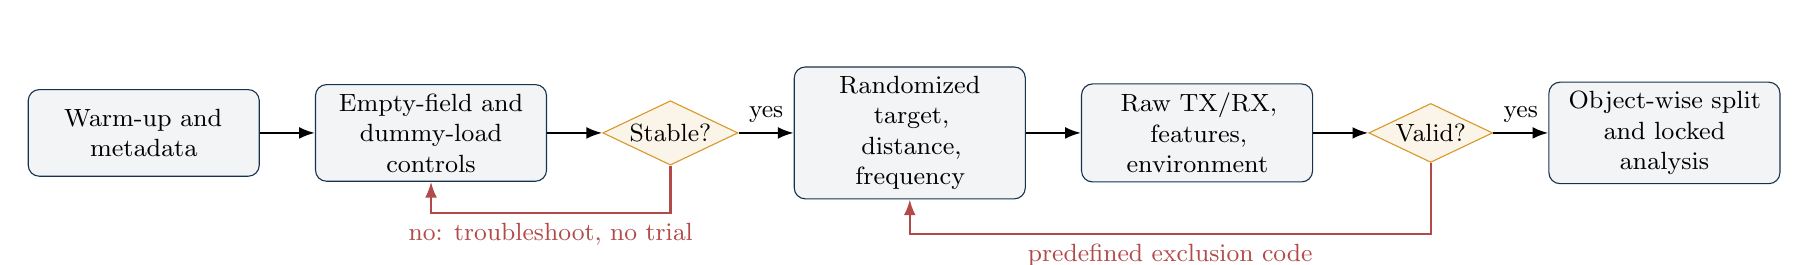
\begin{tikzpicture}[font=\small,node distance=7mm,
 flowstep/.style={draw=navy,rounded corners,minimum height=11mm,align=center,text width=27mm,fill=papergray},
 decision/.style={draw=amber,diamond,aspect=2.1,align=center,inner sep=1pt,fill=amber!10},
 arr/.style={-{Latex[length=2mm]},thick}]
\node[flowstep] (warm) {Warm-up and\\metadata};
\node[flowstep,right=of warm] (noise) {Empty-field and\\dummy-load controls};
\node[decision,right=of noise] (stable) {Stable?};
\node[flowstep,right=of stable] (random) {Randomized target,\\distance, frequency};
\node[flowstep,right=of random] (record) {Raw TX/RX, features,\\environment};
\node[decision,right=of record] (valid) {Valid?};
\node[flowstep,right=of valid] (split) {Object-wise split\\and locked analysis};
\draw[arr] (warm)--(noise); \draw[arr] (noise)--(stable); \draw[arr] (stable)--node[above]{yes}(random); \draw[arr] (random)--(record); \draw[arr] (record)--(valid); \draw[arr] (valid)--node[above]{yes}(split);
\draw[arr,redx] (stable.south) -- ++(0,-.6) -| node[below,pos=.25]{no: troubleshoot, no trial} (noise.south);
\draw[arr,redx] (valid.south) -- ++(0,-.9) -| node[below,pos=.25]{predefined exclusion code} (random.south);
\end{tikzpicture}
}
\caption{Prospective acquisition flow. Stability and validity rules are evaluated without viewing the target label.}
\label{fig:protocol}
\end{figure*}

\subsection{Predefined exclusions and quality control}
Exclude a trial only for: ADC clipping above 0.1\% of samples; TX-current deviation above 5\% from the set point; fixture position error above \SI{1}{\milli\metre}; dropped frames or sample-rate discontinuity; baseline drift above three pre-run standard deviations; or logged protocol violation. Report every exclusion by code and class. No threshold may be tuned on the test objects. A negative-control alarm occurs if the dummy-load condition can be classified above chance using the same pipeline; confirmatory claims are suspended until the leakage path is corrected.

\subsection{Statistical analysis}
All preprocessing is fitted on training data. Continuous features are robust-standardized using the training median and interquartile range. The transparent baseline is nearest centroid; regularized multinomial logistic regression is a secondary model. Hyperparameters are selected by grouped cross-validation, with group equal to physical target identity and acquisition day.

Report the confusion matrix, macro-$F_1$, balanced accuracy, class sensitivity/specificity, calibration error, and 95\% stratified bootstrap confidence intervals. Compare the locked classifier with label permutation ($10{,}000$ permutations). Distance is evaluated by mean and median absolute error, bias, monotonicity violations, and Bland--Altman limits. Contact is scored both per trial and by detection latency. Force, area, and pressure are reported with MAE, RMSE, normalized RMSE, 95th-percentile absolute error, bias, loading/unloading hysteresis, creep, and prediction-interval coverage. Results are stratified by speed, temperature, skin batch, bend state, target class, and contact area. A mixed-effects model assesses mechanism:
\begin{equation}
z_{ijkl}=\beta_0+\beta_1\log d_i+\beta_2 f_j+\beta_3 c_k+\beta_4 m_l+(1|\text{object})+(1|\text{day})+\epsilon,
\end{equation}
where $d$ is distance, $f$ frequency, $c$ target class, and $m$ acquisition mode. Interactions $f\times c$ and chain$\times$c test whether spectral separation survives hardware isolation. Effect sizes and confidence intervals take priority over $p$-values.

Compare four locked models: nearest centroid, regularized linear/logistic baselines, separate single-task compact networks, and the proposed shared multitask network. The multitask claim is supported only if it improves at least one preregistered primary output without violating non-inferiority margins on the others. Evaluate ablations for TX reference, temperature, history, physics loss, uncertainty weighting, and adjacent cells. Selective-risk curves must show error as uncertain predictions are rejected; an OOD test uses entirely unseen people/phantoms, objects, skin batches, and fault states.

\subsection{Power and sample-size strategy}
Because the pilot has no quantitative variance estimate, an honest numerical power calculation is not yet possible. Conduct a separate variance-estimation study whose observations are not reused for confirmatory testing. Then simulate the complete grouped design using the observed object/day covariance and choose sample size for at least 90\% probability that the lower 95\% confidence bound of macro-$F_1$ exceeds 0.50 when the true macro-$F_1$ is 0.75. Publish the simulation code and seed before the confirmatory run.

\section{Expected Failure Modes and Mitigations}
\begin{table*}[t]
\centering\small
\caption{Failure-mode and effects analysis for the proposed skin. Severity (S), occurrence (O), and detectability difficulty (D) are initial ordinal priorities from 1 (low) to 5 (high), not validated reliability statistics.}
\label{tab:fmea}
\begin{tabularx}{\textwidth}{@{}X p{2.9cm}p{1.1cm}p{1.1cm}p{1.1cm}X@{}}
\toprule
Failure mode & Observable consequence & S & O & D & Mitigation / verification\\
\midrule
Codec or power-rail crosstalk & Signal persists with disconnected TX & 3 & 4 & 2 & Independent ADC/DAC supplies; dummy loads; coherence transfer test\\
Body capacitance / grounding & Human dominates all target classes & 4 & 4 & 3 & Electrostatic shield; fixed operator; saline phantom; ground-state factor\\
Coil deformation & Apparent material change during bending & 3 & 4 & 3 & Strain sensor; per-bend calibration; mechanical neutral plane\\
RX saturation and recovery & Bars rail or pulse randomly & 3 & 3 & 2 & Clamp, blanking window, gain staging, saturation-aware feature mask\\
Thermal rise or insulation fault & Unsafe human contact / drift & 5 & 2 & 2 & Current limit, isolation, temperature monitor, dielectric test\\
Domain shift across objects & High training accuracy, poor novel-object accuracy & 4 & 4 & 3 & Split by object; multi-day test; uncertainty rejection\\
Non-monotonic distance response & Unsafe proximity estimate & 5 & 3 & 2 & Monotonicity check; invalidate display; redundant proximity modality\\
Array mutual coupling & Spatial ghosts and channel interference & 3 & 4 & 4 & Sequential scan, calibration matrix, sparse inversion, shielding study\\
\bottomrule
\end{tabularx}
\end{table*}

Three additional coupled hazards require explicit tests. First, force can be correct while pressure is wrong because the inferred contact area is wrong; the pressure head must therefore be disabled whenever area is unobservable. Second, an elastomer can exhibit path-dependent output, so a model trained only on increasing load may underestimate or overestimate unloading force. Third, a high-confidence neural prediction can occur outside the training domain. Skin-batch identity, temperature, diagnostic residuals, ensemble disagreement, and sensor-health flags must participate in an independent validity gate.

The most dangerous error is interpretive: a visually compelling waveform or image can be mistaken for an object ``shape.'' A single coil or single TX--RX pair does not contain sufficient independent spatial measurements for shape reconstruction. Tomographic imaging requires multiple known excitation/receive geometries, a forward model, regularized inversion, and phantom validation \citep{dingley2023emskin}. The optional visual map in the demonstrator should therefore be labeled a time--feature history until an array and reconstruction model exist.

\section{Discussion}
\subsection{What the pilot does and does not support}
The pilot supports the narrow conclusion that the combined hardware/software chain is sensitive to nearby environmental changes. It does not identify which term in \cref{eq:model} caused those changes. The especially strong human response and continued software-parameter dependence without a connected output are classic reasons to test capacitance and codec leakage first. The result may still be useful: a hybrid skin could intentionally exploit capacitive human proximity while using inductive channels for conductive/magnetic targets. Scientific value comes from separating these modalities, not assigning all changes to one mechanism.

The qualitative ranking of gated burst, hybrid, and continuous excitation is likewise provisional. A true conventional pulse-induction metal detector uses a high-current pulse, receiver protection, a blanking interval, and decay sampling after switch-off. A browser audio burst is band-limited, AC-coupled, and low voltage; it is more accurately described as \emph{PI-like gated excitation}. Its apparent advantage may reflect improved baseline rejection or codec behavior rather than classical pulse-induction physics.

\subsection{Path to a distributed robotic skin}
Development should proceed from one characterized element to an array. First establish repeatability and a causal signal path with rigid fixtures. Then test encapsulation and bending, measure mutual-coupling matrices, and introduce sequential scanning. If coil deformation alone proves sufficiently informative, one printed or wound element could span pre-contact and touch with minimal wiring; if it does not, a cell may combine (i) a microcoil impedance channel, (ii) a capacitive proximity electrode, and (iii) an independent force element. Frequency diversity and sensor fusion can then be evaluated with uncertainty-aware models \citep{xu2023ai}. Energy, wiring, and local processing are decisive at robot scale; prior e-skin research shows that distributed coverage can impose substantial system costs \citep{garcia2019energy,someya2019smart}.

Whole-body coverage is especially relevant to service and personal-care robots operating in homes, schools, hospitals, and care facilities. A distributed field can indicate which body region is approaching contact, reduce motion before impact, measure subsequent interaction force, and detect sustained or concentrated pressure. Children, older adults, patients, and people with sensory, cognitive, or mobility limitations are not interchangeable test populations: anatomy, movement, communication, assistive devices, clothing, and acceptable-risk assumptions differ. Initial development should use standardized indenters and tissue phantoms, then consented adults under ethics oversight; studies involving vulnerable participants require a separate justification, safeguarding plan, stopping criteria, and competent supervision.

For gentle contact, the \SIrange{0}{15}{\centi\metre} estimate and learned pressure output must be supervisory cues, not safety-rated measurements. The robot should reduce velocity on conservative proximity thresholds and rely on independent force/torque limits, collision detection, emergency stopping, and application-specific risk reduction. ISO~13482 addresses personal-care robots and physical human--robot contact, with application guidance in ISO/TR~23482-2 \citep{iso13482,isotr23482}. A robot that is itself a medical electrical device may instead fall within medical-device requirements such as IEC~80601-2-78 for rehabilitation, assessment, compensation, or alleviation robots \citep{iec80601}. Applicable standards and regulation depend on intended use and jurisdiction; sensor accuracy alone never establishes compliance. No experiment in this paper authorizes direct human deployment.

\subsection{Limitations}
This study has eight central limitations. First, there is no controlled raw pilot dataset. Second, the audio interface and coil electrical parameters were not fully characterized during the exploratory phase. Third, target geometry and operator position were not controlled. Fourth, the platform's nearest-centroid model is a visualization aid, not a validated classifier. Fifth, browser scheduling and commodity audio processing limit metrological traceability. Sixth, no load-cell, displacement, or contact-area reference has yet been synchronized with the coil, so contact-force and pressure sensing remain hypotheses. Seventh, a scalar cell cannot identify arbitrary contact area, shear force, or pressure distribution without an array or additional modality. Eighth, no training corpus yet represents people, skin batches, temperatures, clothing, assistive devices, ageing, or faults at the breadth required for human-facing deployment. These limitations are made explicit so that future results can be judged against a fixed protocol rather than retrospective interpretation.

\section{Open Science, Ethics, and Safety}
The software, hardware notes, experimental protocol, and LaTeX source are maintained in the public project repository \citep{sensoryskin2026software}. A confirmatory release should add immutable raw PCM or losslessly encoded samples, TX-current traces, session metadata, target photographs/dimensions, calibration records, exclusion logs, and analysis scripts. Each figure derived from data should be generated from a versioned script and manifest.

Human-hand experiments constitute interaction with a person even when no identifying data are intended. Before formal study, obtain the applicable ethics determination or approval, informed consent, and a data-management plan. Do not recruit children, cognitively impaired participants, frail older adults, or patients merely to improve model diversity during feasibility development; use phantoms and low-risk adult studies first. Any later inclusion must be scientifically necessary, independently approved, accessible to the participant, and designed around assent/consent, guardianship where applicable, privacy, fatigue, skin fragility, infection control, and immediate withdrawal. Electrical isolation, leakage current, surface temperature, insulation integrity, cleanability, and fault behavior must be independently reviewed. The system must never connect a power-amplifier output directly to a microphone input and must not serve as the sole protective measure in human--robot interaction.

\section{Conclusion}
Audio-frequency microcoils are a plausible research direction for compliant robotic skin, supported by a wider literature on inductive, magnetic, capacitive, and multimodal tactile systems. Sensory Skin Lab lowers the barrier to investigating that direction by offering local browser acquisition, transparent features, empirical calibration, and structured logging. The proposed extension treats the final approach, first contact, elastomer compression, force, area, and pressure as one gated perception problem and defines a compact uncertainty-aware multitask model suitable for distributed low-cost cells. Its exploratory pilot revealed reproducible-looking environmental sensitivity but also a decisive warning: response persisted when the physical output path was absent, leaving electronic and capacitive confounds unresolved. The appropriate next step is therefore not a stronger claim or amplifier, but a controlled causal experiment with isolated TX/RX chains, dummy loads, instrumented indentation, multiple skin batches, randomized held-out targets, and locked analysis. Only after that test can proximity accuracy, material-response discrimination, force/pressure estimation, array imaging, or safe robotic integration be responsibly claimed.

\section*{Author Contributions}
Francisco Angulo de Lafuente: concept, exploratory investigation, system requirements, software validation, methodology, and manuscript review. The software and manuscript were developed with AI-assisted coding and drafting; the named author remains responsible for experimental accuracy, source verification, and all claims.

\section*{Data and Code Availability}
No controlled dataset is associated with the exploratory observations. Source code and the prospective protocol are available at \url{https://github.com/Agnuxo1/sensory-skin-lab}. A future confirmatory dataset should receive a versioned archival DOI before results are reported.

\section*{Conflict of Interest}
The author declares no known competing financial interest. This statement must be reconfirmed before submission.

\section*{Acknowledgments}
No external funding is claimed. The author acknowledges the open research community whose cited work establishes the scientific context for flexible and robotic skins.

\bibliographystyle{plainnat}
\bibliography{references}

\appendix
\section{Minimum Session Metadata}
Every exported session should contain: UTC timestamp; software and model commits; training-data manifest hash; browser and operating system; input/output device labels and channel mapping; requested and realized sample rate; disabled/enabled audio enhancements; coil identifier and measured $R$, $L$, and self-resonant frequency; skin formulation, batch, cure, thickness, hardness, compression curve, bend state, temperature, and cycle count; TX waveform, frequency, duty cycle, and measured current; preamplifier gain and filters; fixture distance/orientation; indenter identity and area; load-cell and displacement calibration identifiers; target identifier, class, material, dimensions, and temperature; room temperature/humidity; operator location; grounding state; baseline quality; clipping fraction; exclusion code; OOD/validity flags; and randomized trial index.

\section{Prospective Analysis Pseudocode}
\begin{enumerate}
\item Verify file hashes and metadata schema; retain a read-only raw directory.
\item Apply only preregistered validity rules; export the exclusion ledger.
\item Split by physical object and day before fitting preprocessing.
\item Fit robust scaling and the nearest-centroid baseline on training folds.
\item Freeze parameters; evaluate exactly once on held-out objects.
\item Bootstrap at the object level, not the audio-frame level.
\item Run label permutation and dummy-load leakage tests.
\item Evaluate force, area, pressure, hysteresis, creep, and prediction-interval coverage.
\item Run grouped OOD tests across people/phantoms, objects, skin batches, temperatures, and faults.
\item Generate figures and tables from the locked result bundle.
\item Report all planned endpoints, including null and adverse results.
\end{enumerate}

\section{Claim-Evidence Matrix}
\begin{table}[h]
\centering\small
\caption{Permitted wording by evidence level.}
\begin{tabularx}{\linewidth}{@{}p{2.2cm}X X@{}}
\toprule
Level & Permitted statement & Prohibited substitution\\
\midrule
Exploratory observation & ``The displayed receive metric changed when a hand approached.'' & ``The coil detected a human at one metre.''\\
Controlled mechanism & ``The isolated RX response differed from dummy-load controls.'' & ``The mechanism is uniquely inductive'' without modal controls.\\
Held-out classification & ``Macro-$F_1$ was $x$ [CI] on unseen objects.'' & Training accuracy or frame-wise random splits.\\
Calibrated proximity & ``Median error was $x$ cm over 0--15 cm for specified targets.'' & Universal distance range.\\
Calibrated contact force & ``Force NRMSE was $x$ over the stated range, skin and temperature.'' & Universal pressure or safe-touch claim.\\
Calibrated pressure & ``Average pressure error was $x$ for measured contact area.'' & Pressure map from one scalar coil or unknown area.\\
Safety evidence & ``The sensor contributed to a validated safety architecture.'' & ``Safe for human contact'' from sensing accuracy alone.\\
\bottomrule
\end{tabularx}
\end{table}

\end{document}
